\documentclass{frontiersSCNS}
\usepackage{url,hyperref,lineno,microtype,subcaption}
\usepackage[onehalfspacing]{setspace}

\linenumbers

\usepackage[utf8]{inputenc}

\def\keyFont{\fontsize{8}{11}\helveticabold }
\def\firstAuthorLast{Villaseñor-Derbez {et~al.}}
\def\Authors{Juan Carlos Villaseñor-Derbez\(^{1,*}\), Stuart Fulton\(^{2}\), Jorge
Torre\(^{2}\)}
% Affiliations should be keyed to the author's name with superscript numbers and be listed as follows: Laboratory, Institute, Department, Organization, City, State abbreviation (USA, Canada, Australia), and Country (without detailed address information such as city zip codes or street names).
% If one of the authors has a change of address, list the new address below the correspondence details using a superscript symbol and use the same symbol to indicate the author in the author list.
\def\Address{\(^{1}\)Bren School of Environmental Science and Management, University
of California, Santa Barbara, Santa Barbara, CA,
USA\newline \(^{2}\)Comunidad y Biodiversidad A.C., Guaymas, Mexico}
% The Corresponding Author should be marked with an asterisk
% Provide the exact contact address (this time including street name and city zip code) and email of the corresponding author
\def\corrAuthor{Juan Carlos Villaseñor-Derbez, Bren Hall, University of California,
Santa Barbara, Santa Barbara, CA, 93106}

\def\corrEmail{\href{mailto:jvillasenor@bren.ucsb.edu}{\nolinkurl{jvillasenor@bren.ucsb.edu}}}

\begin{document}
\onecolumn
\firstpage{1}

\title[Mexican marine reserves]{Community-based marine reserves produce biological and economic benefits} 

\author[\firstAuthorLast ]{\Authors} %This field will be automatically populated
\address{} %This field will be automatically populated
\correspondance{} %This field will be automatically populated

\extraAuth{}

\maketitle



\section{Introduction}\label{introduction}

La sobrepesca y prácticas pesqueras no sostenibles son unas de las
mayores amenazas para la conservación de los ecosistemas marinos del
mundo \citep{halpern_2008-dK,halpern_2017-Zi}. La implementación de
reservas marinas (\emph{i.e.} áreas donde la captura de una o más
especies está prohibida) es una medida de manejo frecuentemente
propuesta para recuperar stocks pesqueros e impulsar la productividad
pesquera en aguas cercanas
\citep{afflerbach_2014-HP,krueck_2017-J1,sala_2017-69}. Recientes
trabajos han demostrado que también pueden mitigar y proveer
amortiguamiento ante el cambio climático \citep{roberts_2017-J9},
variabilidad ambiental \citep{micheli_2012-EU}, resolver problemas de
pesca incidental \citep{hastings_2017-sm} y, en general, incrementar la
biomasa, riqueza y densidades de organismos dentro de sus fronteras
\citep{lester_2009-Ks,giakoumi_2017-V2,sala_2017-69}.

En México, las reservas marinas han sido comúnmente establecidas como
zonas núcleo dentro de Reservas de la Biósfera (RBs), administradas por
la Comisión Nacional de Áreas Naturales Protegidas (CONANP). Al día de
hoy, 36 RBs protegen una porción del ambiente marino en México. Sin
embargo, solamente 26 de estas incluyen (pequeñas) zonas núcleo donde
las actividades pesqueras están prohibidas. Aunque la CONANP ha hecho
esfuerzos importantes por involucrar a los actores durante la
implementación de las reservas, esto aún se caracteriza por un proceso
descendente, el cual conlleva a la falta de cumplimiento por parte de
los actores. La escasez de recursos monetarios y humanos de la limitan
también el monitoreo y vigilancia de las reservas, y a su vez, el
desempeño de la reserva.

Buscando promover una alternativa con procesos ascendentes para
implementar reservas marinas, las Organizaciones de la Sociedad Civil
(OSCs) comenzaron a trabajar con comunidades pesqueras para establecer
reservas comunitarias \citep{uribe_2010-u2} . Estas son comúnmente
establecidas dentro de zonas de concesión, una forma de derechos de uso
territoriales para pesquerías (TURF, en inglés). Al permitir a los
pescadores diseñar sus propias reservas, una mayor proporción de la
comunidad está de acuerdo con los perímetros y reglas establecidas, y
por lo tanto los respetan
\citep{gelcich_2015-Gw,espinosaromero_2014-PY,beger_2004-Y8} .
Adicionalmente, los pescadores pueden implementar sus reservas por un
periodo acordado (usualmente cinco años), después del cual la reserva
puede ser abierta a la pesca. Esto provee a los pescadores con un
sentido de confianza de que, en caso de ser necesario, aún tienen acceso
a pescar esa zona. Las reservas son directamente vigiladas y
monitoreadas por la comunidad, quienes comúnmente utilizan pequeñas
embarcaciones (\emph{e.g.} pangas) para patrullar la zona, o realizan
avistamientos desde la costa en búsqueda de pescadores ilegales Aún así,
las reservas comunitarias carecen de reconocimiento legal; por lo tanto,
no hay forma de penalizar a los infractores.

Sin embargo, en el 2014 una nueva norma \citep{nom} permite a los
pescadores solicitar el establecimiento de reservas marinas bajo el
nombre de ``Zonas de refugio Pesquero'' (ZRP). El manejo de las ZRP
combina procesos ascendentes y descendentes al reconocer legalmente las
reservas propuestas por las comunidades. Posterior a la revisión por
parte de la Comisión Nacional de Acuacultura y Pesca (CONAPESCA) y la
opinión técnica del Instituto Nacional de Acuacultura y Pesca (INAPESCA)
las ZRP son establecidas por el periodo solicitado por los pescadores.
El monitoreo y la vigilancia de las ZRP es típicamente llevado a cabo
por la comunidad , con ayuda de OSCs locales. Hasta este cambio
regulatorio, las reservas comunitarias no contaban con el soporte legal,
y eran solamente reconocidas por la comunidad. Al día de hoy, existen 39
ZRP establecidas en el Pacífico, Golfo de California y Caribe Mexicano.

Aunque existen tres aproximaciones generales para implementar reservas
marinas en México (\emph{i.e.} Zonas núcleo dentro de AMP, reservas
comunitarias y Zonas de Refugio Pesquero), aún no comprendemos a fondo
las características sociales que permiten su efectividad. La ciencia de
reservas marinas se ha enfocado ampliamente en los efectos biológicos
que estas tienen
\citep{lester_2009-Ks,giakoumi_2017-V2,sala_2017-69,afflerbach_2014-HP,krueck_2017-J1}.
Aunque el aspecto ecológico de las reservas es importante para su éxito,
su efectividad también depende del estado socioeconómico y los sistemas
de gobernanza de las comunidades pesqueras.

La literatura indica que diferentes características influyen en el éxito
de una reserva. En Palau, por ejemplo, la edad (\emph{i.e.} tiempo
transcurrido desde implementación), tamaño y hábitat contenido son
características claves que determinan la efectividad
\citep{friedlander_2017-oI}. Por otro lado, en el Mar Mediterráneo,
\citet{difranco_2016-Xw} identifican que la procuración y vigilancia,
presencia de un plan de manejo, participación de pescadores en el
manejo, representación de pescadores en la toma de decisiones y
promoción de la pesca sustentable son los cinco factores que incrementan
la salud de los stocks y el ingreso económicos a los pescadores, a la
vez que se presenta una mayor aceptación social de las prácticas de
manejo. En una aproximación global, \citet{edgar_2014-UO} encuentran que
la procuración, edad, tamaño y aislamiento son determinantes de la
efectividad de las reservas. Por lo tanto, observamos que las
características que habilitan el éxito varían a través de regiones, y
poco esfuerzo se ha hecho por comprender estas interacciones en México.

El objetivo de este trabajo este trabajo es realizar una evaluación de
la efectividad de reservas marinas en México, presentando resultados de
cinco comunidades costeras como caso de estudio. Con el fin de obtener
una visión holística del sistema, la evaluación se realizará tomando en
cuenta indicadores biológicos, socioeconómicos y de gobernanza. La
evaluación de éstos cinco casos de estudios nos permitirá identificar la
manera en que las características socioeconómicas y de gobernanza se
relacionan con la efectividad (biológica) de las reservas marinas
evaluadas. Los patrones identificados podrán utilizarse para informar la
toma de decisiones para la implementación de la red de reservas marinas
en la Región de las Grandes Islas del Golfo de California.

\section{Materials and Methods}\label{materials-and-methods}

\subsection{Study area}\label{study-area}

Las comunidades utilizadas en este reporte se distribuyen a lo largo de
la costa Pacífica de Baja California (n = 1) y el Sistema Arrecifal
Mesoamericano (n = 2; Fig \ref{fig:map}).

\subsubsection{Isla Natividad}\label{isla-natividad}

La Isla Natividad se encuentra en la costa oeste de la Península de Baja
California, donde el hábitat predominante es el bosque de kelp o sargazo
gigante (\emph{Macrocystis pyrifera}) y los arrecifes rocosos. En la
isla, la Sociedad Cooperativa de Producción Pesquera (SCPP) Buzos y
Pescadores de la Baja California SCL realiza actividades de extracción
de los recursos marinos. Aunque la langosta roja (\emph{Panulirus
interruptus}) es la especie más importante en términos económicos, otras
especies importantes incluyen la escama (con un enfoque en Jurel;
\emph{Seriola lalandi}), el pepino de mar (\emph{Parastichopus
parvimensis}), el erizo rojo (\emph{Mesocentrotus franciscanus}), el
caracol (\emph{Megastraea turbanica} y \emph{M. undosa}) y, hasta el
2010, el abulón (\emph{Haliotis sp.}). En 2006, por medio de un proceso
participativo, la cooperativa decidió establecer dos reservas marinas de
manera voluntaria. Agentes externos a la cooperativa, como personal de
Comunidad y Biodiversidad A.C., académicos de la Universidad de
Stanford, y personal de la CONANP (de la oficina de Reserva de la
Biósfera El Vizcaíno), también participaron en el diseño e
implementación de las reservas. Las reservas fueron establecidas como
instrumento de manejo pesquero, buscando recuperar las poblaciones de
abulón y otros invertebrados. Al día de hoy, las reservas marinas de
Isla Natividad no han recibido reconocimiento legal, pero la cooperativa
ha mostrado interés por reconocerlas como Zonas de Refugio Pesquero
(ZRP). Los pescadores tienen un sistema de turnos para vigilar la
reserva día y noche desde embarcaciones patrulla.

\subsubsection{María Elena}\label{maria-elena}

María Elena es una comunidad pesquera en la costa de Quintana Roo. Los
arrecifes coralinos y manglares son los principales ecosistemas
representados en la zona. El campo pesquero es utilizado por pescadores
de la SCPP Cozumel scl (de la Isla de Cozumel). La principal especie
aprovechada por ésta organización es la langosta espinosa del caribe
(\emph{Panulirus argus}). La cooperativa cuenta con permiso de pesca de
escama y concesión de langosta. En el 2012, la Cooperativa, en conjunto
con la Alianza Kanan Kay, COBI, CONANP, CONAPESCA, Oceanus, Fundación
Claudia y Roberto Hernández, Fundación Haciendas del Mundo Maya,
establecieron ocho ZRP con una vigencia de cinco años. La vigilancia de
las reservas se realiza por medio del equipo de vigilancia comunitaria,
con apoyo de la CONANP y una embarcación -donada por COBI- utilizada
para realizar recorridos frecuentes.

\subsubsection{Punta Herrero}\label{punta-herrero}

La comunidad de Punta Herrero se encuentra aproximadamente a 15 km al
sur del campo pesquero de María Elena. De igual manera, los arrecifes
coralinos y manglares son los principales ecosistemas representados en
la zona, y la principal especie explotada es la langosta. Sin embargo,
la SCPP José María Azcorra también cuenta con permisos para pesca de
escama y tiburón y una concesión de langosta. En una réplica del
ejercicio realizado en María Elena -con presencia de los mismos
actores-, cuatro ZRP fueron establecidas en el 2013, con una vigencia de
cinco años. El equipo de vigilancia comunitaria, con apoyo de la CONANP,
se encarga de la vigilancia de las reservas.

\begin{figure}
\centering
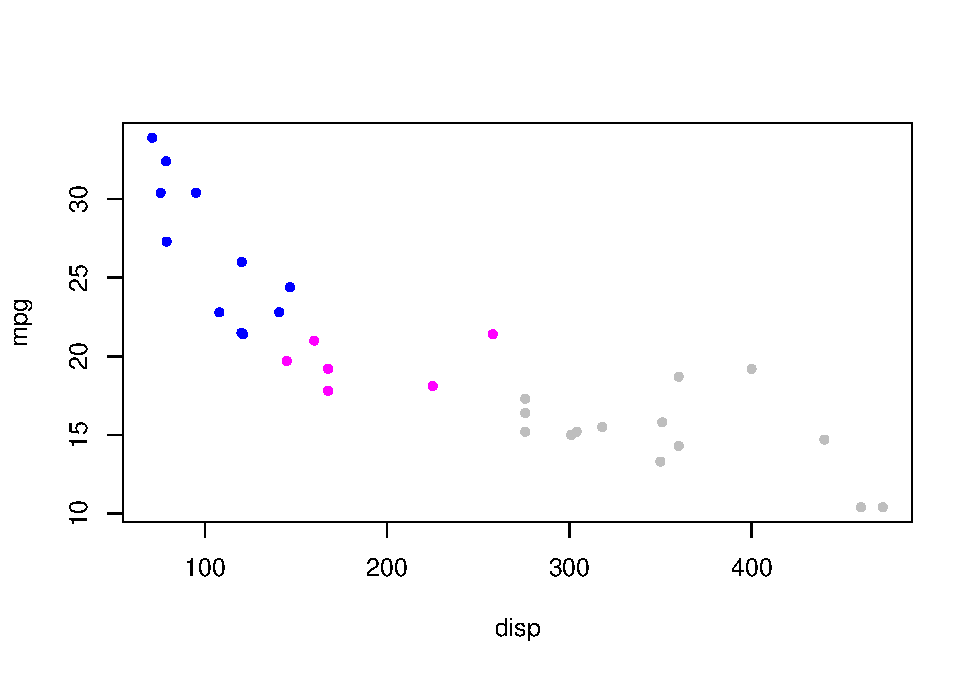
\includegraphics{Villasenor-Derbez_files/figure-latex/unnamed-chunk-1-1.pdf}
\caption{\label{fig:unnamed-chunk-1}\label{fig:map}Mapa de la localización
general de las comunidades de estudio. El panel de la derecha es un
acercamiento a las comunidades de María Elena y Punta Herrero.}
\end{figure}

\subsection{Data collection}\label{data-collection}

Para evaluar las reservas, utilizamos tres fuentes de información. La
información ecológica proviene de los monitoreos ecológicos realizados
anualmente en las zonas reserva y control. Cada año, se realizan censos
visuales para evaluar las comunidades de peces e invertebrados,
registrando riquezas, abundancias y tallas (en peces). Esta información
nos permite calcular los indicadores biológicos de manera anual. Al
tener valores de diferentes indicadores biológicos antes y después de la
implementación de las reservas, para las zonas de reserva y sitios
control, tenemos un diseño muestreal de Antes-Después-Control-Impacto.

También incluimos información socioeconómica relevante proveniente de
los avisos de arribo de CONAPESCA. En este caso, se tienen registros
mensuales de los recursos aprovechados por las diferentes comunidades,
en los que se reportan los arribos (Toneladas) y el valor de los arribos
(\$). La información se encuentra disponible para el periodo 2001 -
2014. Ya que las categorías registradas por CONAPESCA son amplias y
existe un nivel de error, utilizamos únicamente los arribos reportados
para langosta entera fresca a nivel de cooperativa. Los ingresos
generados por arribos son ajustados por medio del índice de precio al
consumidor.

La información de gobernanza fue obtenida a nivel de comunidad, pidiendo
a personas familiares con las comunidades que proveyeran la información
necesaria. La información de gobernanza no es evaluada de manera
cuantitativa. En su lugar, esta se interpreta de manera tal que podamos
comprender qué decisiones, reglas y estructuras tienen un impacto en la
reserva.

\subsection{Data analysis}\label{data-analysis}

Dada la similitud de objetivos entre las reservas, la evaluación se
realiza con los mismos indicadores. En este caso, se utilizan 6
indicadores biológicos, 2 socioeconómicos y 5 de gobernanza (Tabla
\ref{table:indicators}). Según la disponibilidad de datos, se calculó la
densidad de las especies objetivo presentadas en la sección de
descripción de las comunidades. El criterio de selección fue que cada
especie debía tener, por lo menos, dos observaciones anuales para las
zonas de reserva y control.

\begin{table}

\caption{\label{tab:unnamed-chunk-2}\label{table:indicators}Lista de indicadores utilizados para evaluar resvas marinas, agrupados por tipo.}
\centering
\begin{tabular}[t]{l|l}
\hline
Category & Indicador\\
\hline
Biological & Índice de diversidad de shannon\\
\hline
 & Riqueza\\
\hline
 & Densidad\\
\hline
 & Nivel trófico\\
\hline
 & Biomasa\\
\hline
 & Densidad de especies objetivo\\
\hline
Socioeconomic & Ingresos por especies objetivo\\
\hline
 & Arribos de especies objetivo\\
\hline
Governance & Tipo de acceso a la pesquería\\
\hline
 & Grado de pesca ilegal\\
\hline
 & Procuración de la reserva\\
\hline
 & Tipo de organización pesquera\\
\hline
 & Edad de la reserva\\
\hline
\end{tabular}
\end{table}

\subsubsection{Biological}\label{biological}

Utilizando un análisis de diferencia en diferencias podemos estimar el
efecto que la reserva tienen en los indicadores biológicos
\citep{moland_2013-VP} con el uso de un modelo de regresión lineal
múltiple:

\[I = \beta_0 + \sum \gamma Year + \beta_1 Zona + \sum \lambda Year\times Zona + \Omega + \epsilon\]

En este caso, modelamos los años como factores, tomando como referencia
el primer año en la serie de datos de cada comunidad. Modelar los años
como factores reduce la estructura del modelo, y relaja el ajuste al no
asumir una tendencia lineal entre años; es decir, el cambio observado
entre 2006 - 2007 no deberá de ser igual al observado entre el 2009 -
2010. Incluimos también un término para la zona, en la que la variable
toma un valor de 0 si el sitio es una zona control y de 1 si es una zona
de reserva. Finalmente, incluimos un término de interacción entre la
variable de Zona y el Año. En este modelo, \(\lambda_i\) representa el
efecto que la reservas tuvo sobre un indicador en cada año y con
respecto a los sitios control. El termino \(\Omega\) captura efectos
fijos por especies y por sitio.

\subsubsection{Socioeconomic}\label{socioeconomic}

El análisis de datos socioeconómicos se aplicó únicamente a Isla
Natividad, María Elena y Punta Herrero, siguiendo un modelo con la
forma:

\[I = \beta_0 + \beta_1Post\]

Que nos permite comparar el cambio en el promedio de los indicadores
antes (Post = 0) y después (Post = 1) de la implementación de la
reserva. Tanto para los indicadores biológicos como los socioeconómicos,
los coeficientes fueron ajustador con el estimador de muestras
heterocedásticas.

\subsubsection{Governance}\label{governance}

\section{Results}\label{results}

A continuación se presentan los resultados de cada una de las
comunidades. Los resultados biológicos se presentarán para cada
comunidad, discutiendo primero los indicadores en común con otras
comunidades (Shannon, Riqueza, Densidad, Nivel Trófico, Biomasa para
peces e invertebrados) y, según su caso, las densidades de las especies
objetivo. Habiendo presentado los resultados biológicos, nos enfocaremos
después en los socioeconómicos y de gobernanza. Usaremos esta
información para identificar las causas (sociales) del éxito (biológico)
de las reservas.

\begin{figure}
\centering
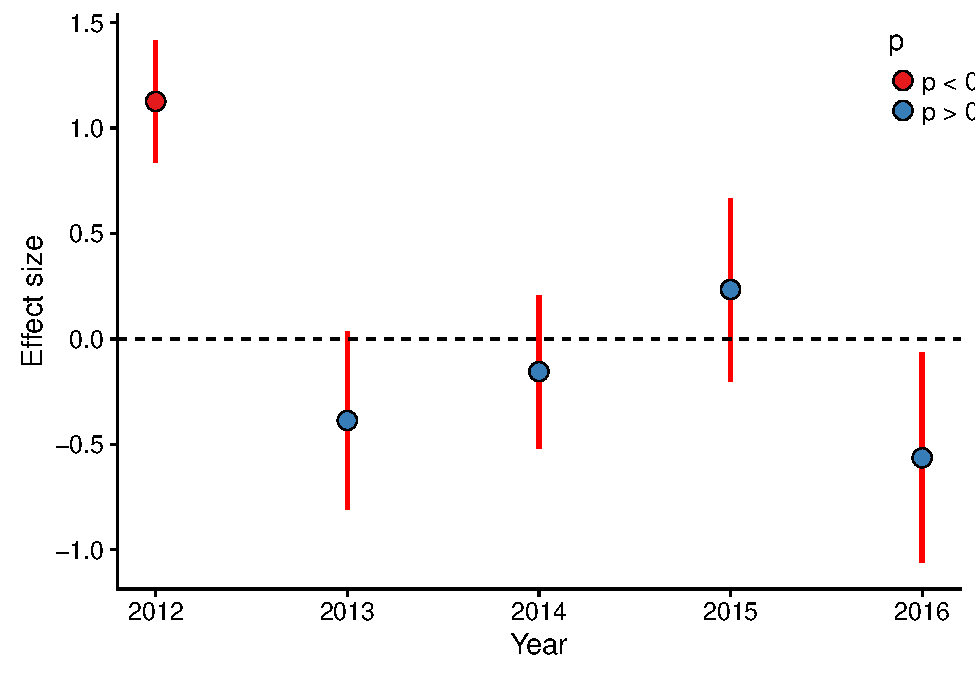
\includegraphics{Villasenor-Derbez_files/figure-latex/unnamed-chunk-3-1.pdf}
\caption{\label{fig:unnamed-chunk-3}\label{fig:indicators}Effect sizes for
marine reserves from Isla Natividad (IN; red cirlcles), Maria Elena (ME;
blue triangles), and Punta Herrero (PH; green squares). Plots are
ordered by survey type (left: fish; right: invertebrates) and
indicators: Abundance (A, B), Richness (C, D), and Shannon's diversity
index (E, F)}
\end{figure}

\section{Discussion}\label{discussion}

\section*{Conflict of Interest Statement}

The authors declare that the research was conducted in the absence of
any commercial or financial relationships that could be construed as a
potential conflict of interest.

\section*{Author Contributions}

JC analyzed and interpreted data, discussed the results and wrote the
manuscrip. SF and JT edited the manuscript and discussed the results.

\section*{Funding}

Details of all funding sources should be provided, including grant
numbers if applicable. Please ensure to add all necessary funding
information, as after publication this is no longer possible.

\section*{Acknowledgments}

This is a short text to acknowledge the contributions of specific
colleagues, institutions, or agencies that aided the efforts of the
authors.

\section*{Supplemental Data}

\href{http://home.frontiersin.org/about/author-guidelines#SupplementaryMaterial}{Supplementary Material}
should be uploaded separately on submission, if there are Supplementary
Figures, please include the caption in the same file as the figure.
LaTeX Supplementary Material templates can be found in the Frontiers
LaTeX folder

\paragraph*{S1 Figure}
\label{S1_Figure}

Maps of the marine reserves and corresponding control sites at each
community.

\paragraph*{S2 Table}
\label{S2_Table}

Table with a general overview of on the governance characteristics of
each community.

\bibliographystyle{frontiersinSCNS_ENG_HUMS}\bibliography{references}

\section*{Figure captions}



\end{document}
